\documentclass[12pt, letterpaper]{report}

\title{\textbf{ECS 132 Term Project}}
\author{\parbox{\linewidth}{\centering%
  Steven Alvarado, Russell Chien, and Ruth Hailu\endgraf\bigskip
  University of California, Davis}}

\usepackage{datetime}
\newdateformat{monthyeardate}{\monthname[\THEMONTH] \THEYEAR}
\date{\monthyeardate\today}

\usepackage{graphicx} 
\usepackage{titlesec}
\usepackage{amsmath}
\usepackage{listings}
\usepackage[usenames,dvipsnames]{color} 

\lstset{ 
  language=R,                    	 	 % The language of the code
  basicstyle=\normalsize\ttfamily,		 % The size of the fonts that are used for the code
  numbers=left,                   		 % Where to put the line-numbers
  numberstyle=\normalsize\color{Blue},  % The style that is used for the line-numbers
  stepnumber=1,                   		 % The step between two line-numbers. If it is 1, each line
                                  			 % will be numbered
  numbersep=5pt,                  		 % How far the line-numbers are from the code
  backgroundcolor=\color{white},  	 % Choose the background color. You must add \usepackage{color}
  showspaces=false,               		 % Show spaces adding particular underscores
  showstringspaces=false,         		 % Underline spaces within strings
  showtabs=false,                 		 % Show tabs within strings adding particular underscores
  frame=single,                   		 % Adds a frame around the code
  rulecolor=\color{black},        		 % If not set, the frame-color may be changed on line-breaks within not-black text (e.g. commens (green here))
  tabsize=2,                      			 % Sets default tabsize to 2 spaces
  captionpos=b,                   		 % Sets the caption-position to bottom
  breaklines=true,                		 % Sets automatic line breaking
  breakatwhitespace=false,        		 % Sets if automatic breaks should only happen at whitespace
  keywordstyle=\color{RoyalBlue},      	 % Keyword style
  commentstyle=\color{YellowGreen},     % Comment style
  stringstyle=\color{ForestGreen}      	 % String literal style
} 

\graphicspath{{plots/}}
\titleformat{\chapter}[display]
  {\normalfont\huge\bfseries\filcenter}{\chaptertitlename\ \thechapter}{20pt}{\Huge}
\titlespacing*{\chapter}
  {0pt}{30pt}{20pt}

\begin{document}
\maketitle



\chapter{The Normal Family}
\section{Communities and Crime: pctWWage}
Our group observed that the variable \textbf{pctWWage} of the Communities and Crime dataset seemed well-approximated by the normal family of continuous distributions.
According to the UCI Machine Learning Repository, \textbf{pctWWage} is described as the percentage of households within the United States with wage or salary income in 1989.

\section{Histogram and Density}
Below are the histogram and density plots of pctWWage, generated using R's hist(), plot(), and density() functions.
\begin{center}
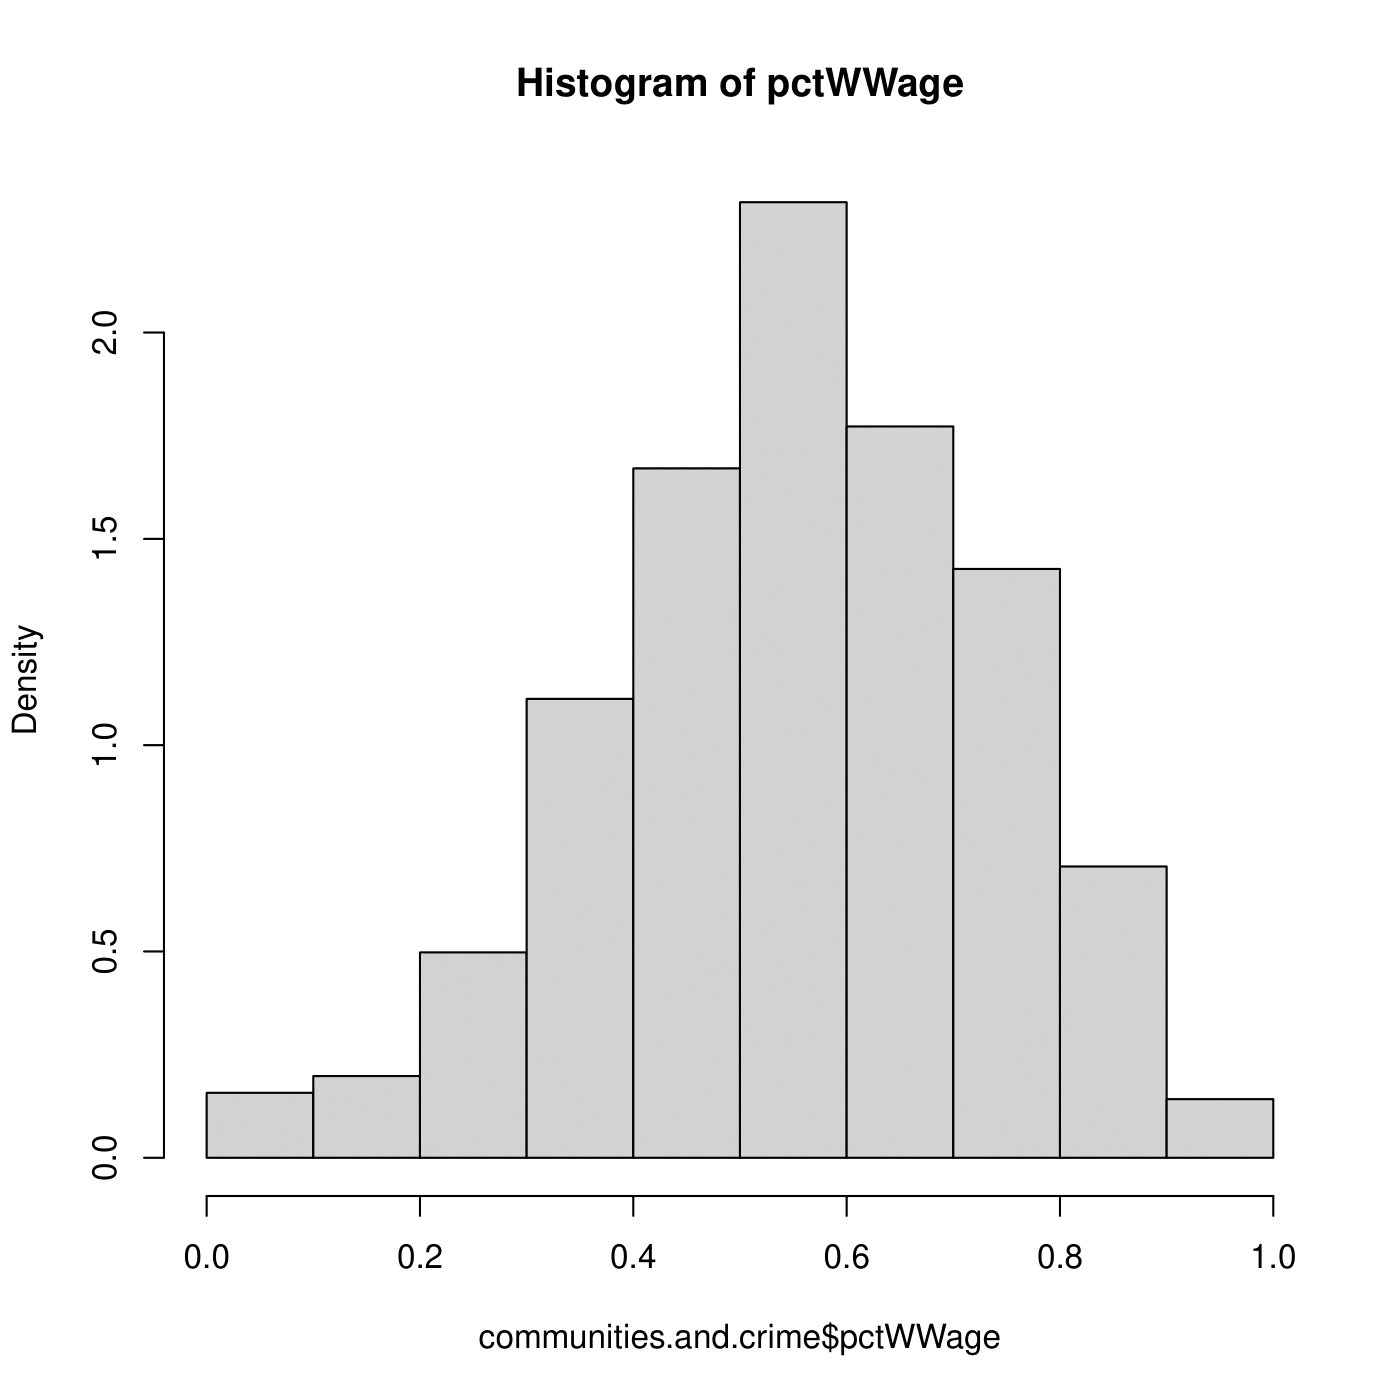
\includegraphics[width=0.45\textwidth]{normal/pctWWage_hist}
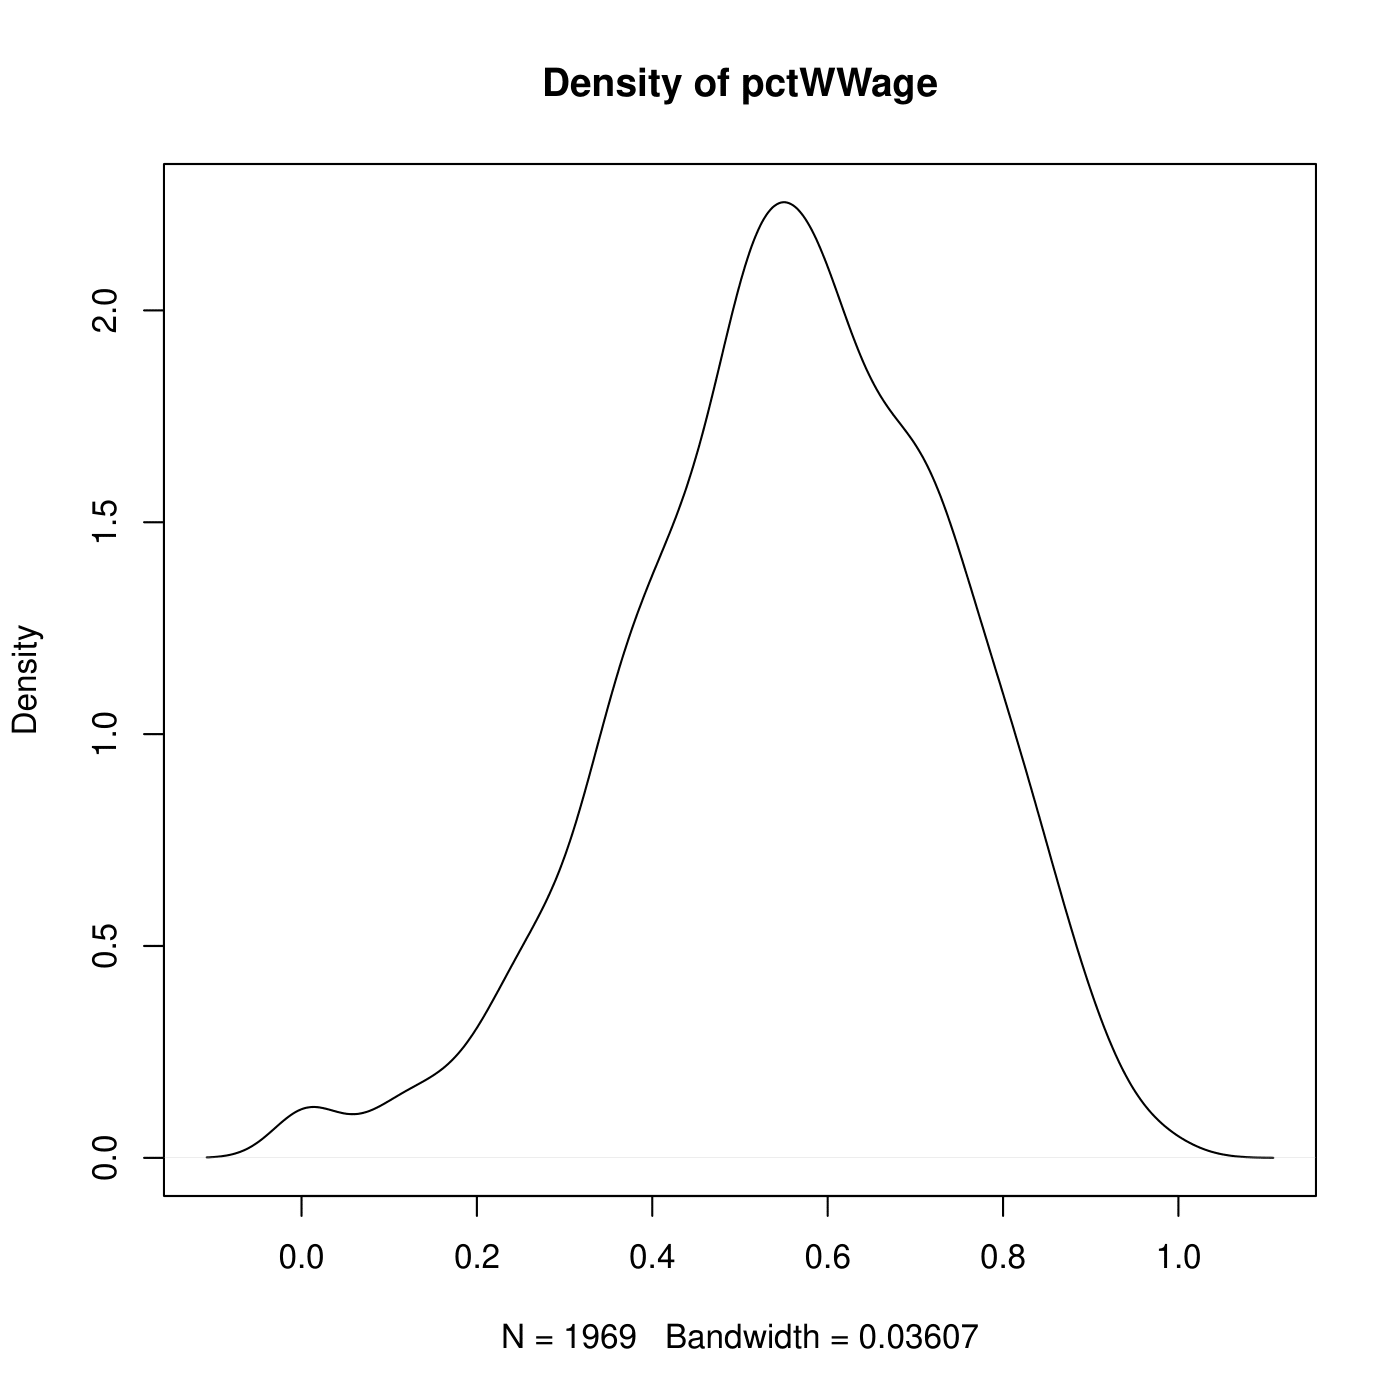
\includegraphics[width=0.45\textwidth]{normal/pctWWage_density}
\end{center}

\pagebreak
\section{Maximum Likelihood Estimation}
To find the MLE of pctWWage, we first defined our log-likelihood function as:
\begin{equation}
  LL(\mu, \sigma^2) = -n \log{(2\pi)} + \frac{\log{(\sigma^2)}}{2} - \frac{\sum(x-\mu)^2}{2\sigma^2}
\end{equation}

Using R's built-in mle() function, we utilized the \textit{negative} log-likelihood function to find the normal parameters of pctWWage.
\begin{lstlisting}
z <- mle(minuslogl = ll, start = c(list(mean = 1), list(var = 1)))
\end{lstlisting} 

Superimposing the resulting density on pctWWage's kernel plot results in the graph:
\begin{center}
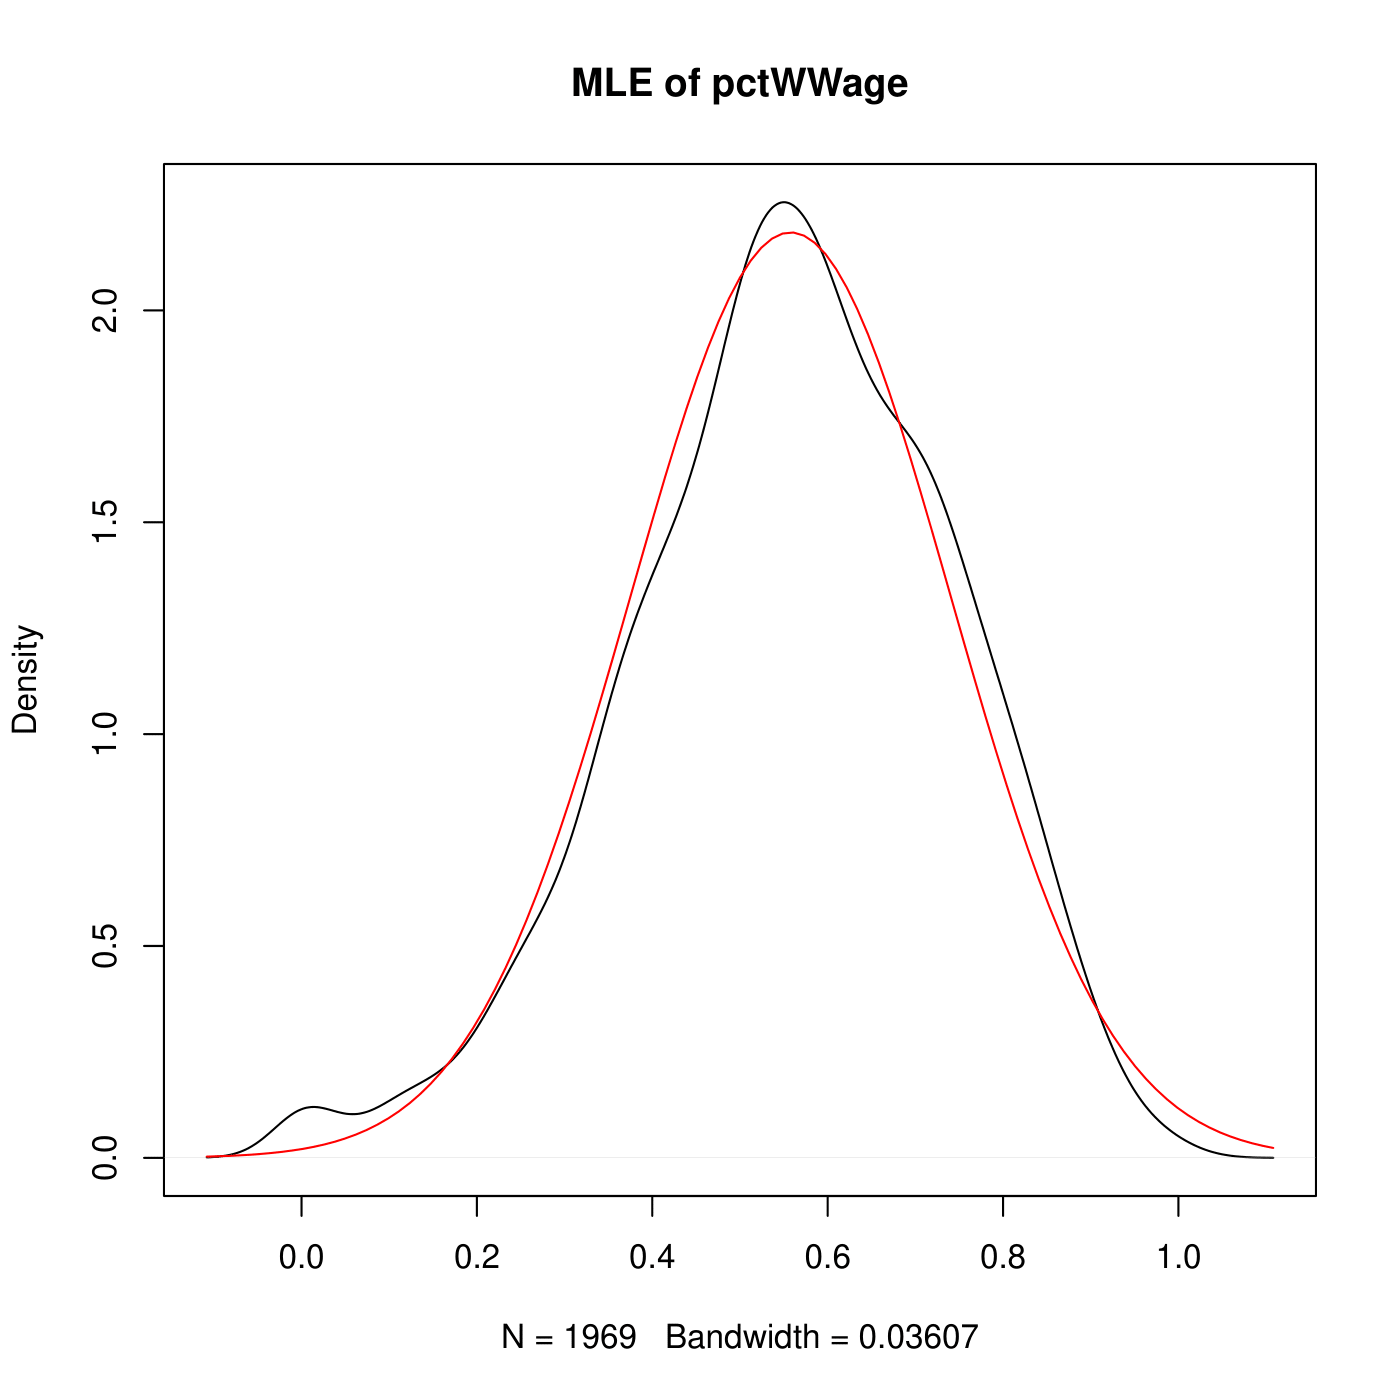
\includegraphics[width=0.45\textwidth]{normal/pctWWage_mle}
\end{center}

\pagebreak
\section{Method of Moments}
To find the MM-estimated density of pctWWage, we used the following function to predict the values of $\mu$ and $\sigma^2$:
\begin{lstlisting}
  mm <- function(x) {
    mu <- mean(x)
    sigma <- sqrt(mean(x^2) - mu^2)
    return(c(mu, sigma))
  }  
\end{lstlisting} 

Superimposing the resulting density results in the graph:
\begin{center}
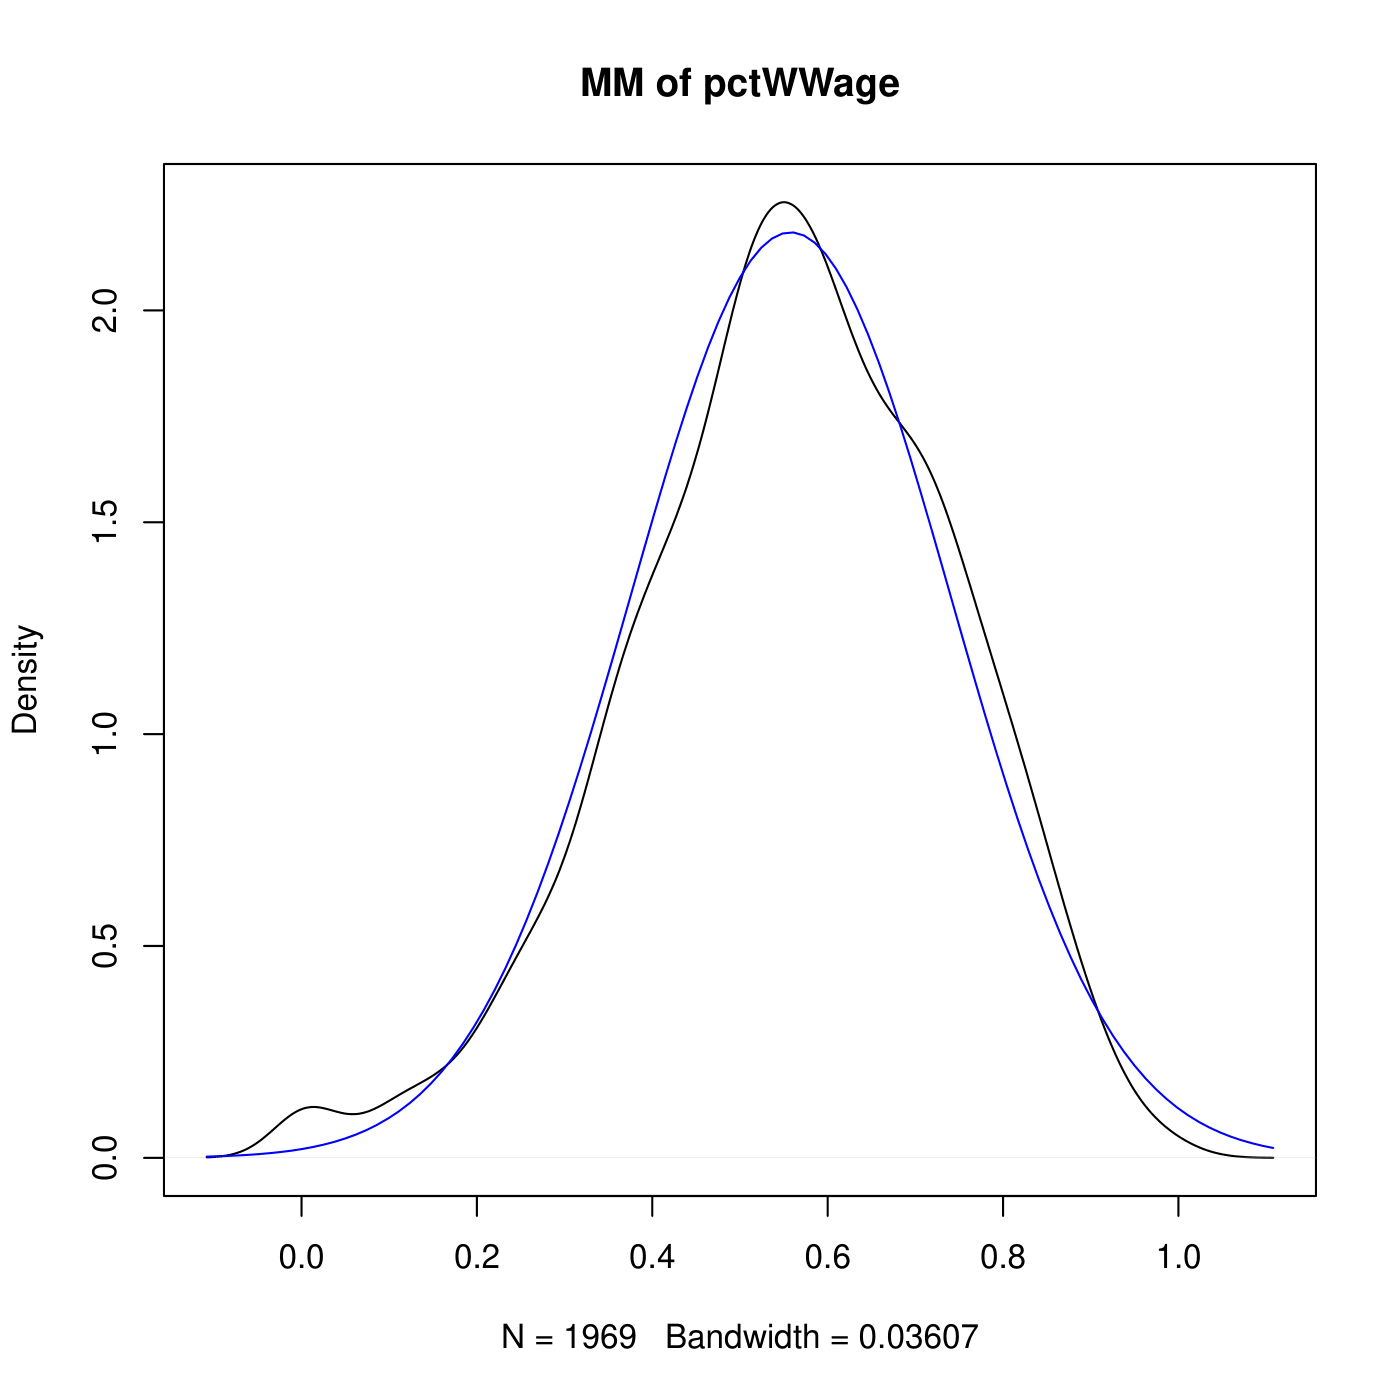
\includegraphics[width=0.45\textwidth]{normal/pctWWage_mm}
\end{center}

\section{Analysis}
The MLE and MM normal approximations appear to be a good fit for pctWWage's data. The density estimates obtained from both methods closely align with the density curve derived directly from the dataset. 
Thus, our group can confidently conclude that the variable pctWWage is well-approximated by the normal distribution family.



\maketitle
\chapter{The Exponential Family}
\section{Communities and Crime: PctLargHouseFam}

For the exponential family of continuous distributions, we observed that the variable \textbf{PctLargHouseFam} could potentially be a suitable approximation. 
The UCI ML Repo describes \textbf{PctLargHouseFam} as the percentage of family households with six or more family members. 

\section{Histogram and Density}
Below are the histogram and density plots of PctLargHouseFam, using similar methods of generation as the previous section.
\begin{center}
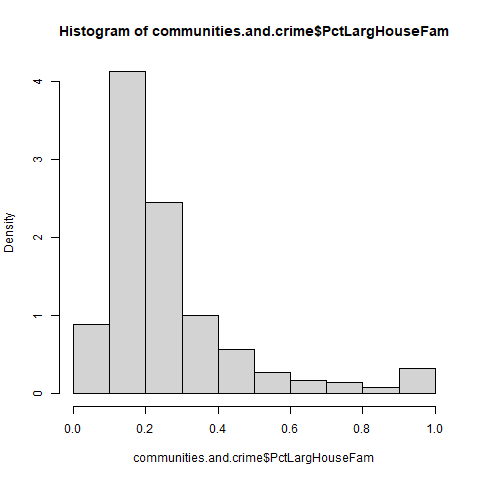
\includegraphics[width=0.45\textwidth]{exponential/PctLargHouseFam_hist}
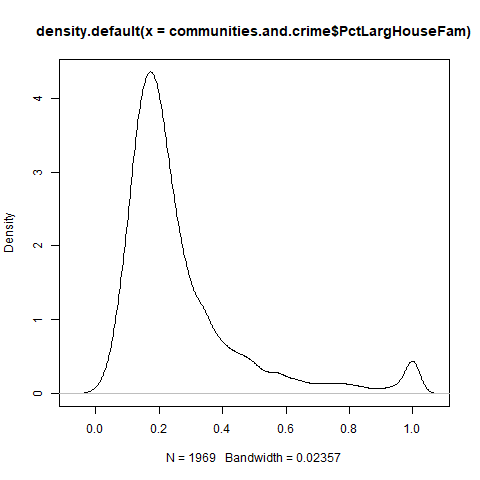
\includegraphics[width=0.45\textwidth]{exponential/PctLargHouseFam_density}
\end{center}

\pagebreak
\section{Maximum Likelihood Estimation}
To find the MLE of PctLargHouseFam, we defined our log-likelihood function as:
\begin{equation}
 LL(\lambda) = n \log{\lambda} - \lambda \sum{x}
\end{equation}

Using R's built-in mle() function, we utilize the \textit{negative} log-likelihood function to find the exponential parameters of PctLargHouseFam:
\begin{lstlisting}
  z <- mle(minuslogl = ll, start = c(list(lambda = 1)))
\end{lstlisting} 

\begin{center}
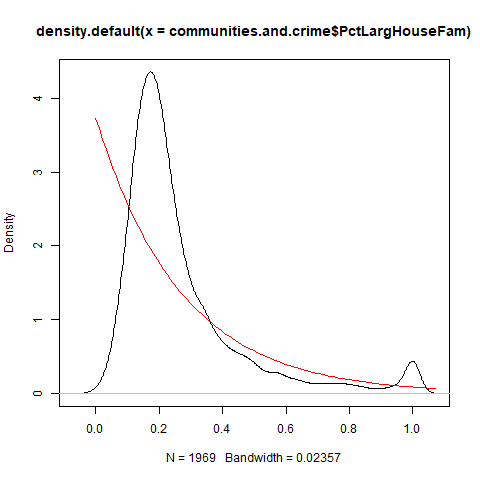
\includegraphics[width=0.45\textwidth]{exponential/PctLargHouseFam_mle}
\end{center}

\pagebreak
\section{Method of Moments}
To find the MM-estimated density of PctLargHouseFam, we used the following function to predict $\lambda$:
\begin{lstlisting}
  mm <- function(x) {
    lambda <- 1 / mean(x)
    lambda
}
\end{lstlisting}

\begin{center}
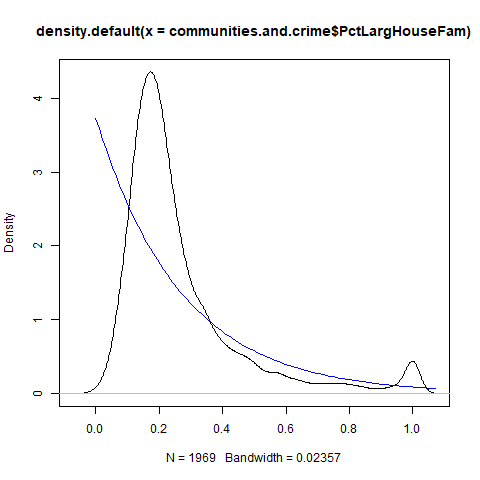
\includegraphics[width=0.45\textwidth]{exponential/PctLargHouseFam_mm}
\end{center}

\section{Analysis}
The exponential approximation shows a reasonable fit at the tail end of the density distribution, but it exhibits noticeable deviations from the actual data around \(x=0.2\).
The exponential distribution assumes a constant and consistent decay rate, which does not accurately capture the characteristics of the data around its peak.



\maketitle
\chapter{The Gamma Family}
\section{Communities and Crime: PctNotHsGrad}

Our group observed that the gamma family of continuous distributions seemed to well-approximate the variable \textbf{PctNotHsGrad}.
On the UCI ML Repo, \textbf{PctNotHsGrad} is defined as the percentage of people 25 and over that are not high school graduates.

\section{Histogram and Density}
Below are the histogram and density plots of PctNotHsGrad.
\begin{center}
\includegraphics[width=0.45\textwidth]{gamma/PctNotHsGrad_hist}
\includegraphics[width=0.45\textwidth]{gamma/PctNotHsGrad_density}
\end{center}

\pagebreak
\section{Maximum Likelihood Estimation}
To find the MLE of the gamma family, we first defined our log-likelihood function as:
\begin{equation}
  LL(k, \theta) = (k-1)\sum(\log{x}) - \sum(\frac{x}{\theta}) - n k \log{(\theta)} - n \log{(\Gamma(k))}
\end{equation}
We then had to scale our data to ensure the log-likelihood function remained finite: 
\begin{lstlisting}
  x[which(x == 0)] <- 0.0001  
\end{lstlisting} 

Using R's built-in mle() function, we utilized the \textit{negative} log-likelihood function to find the gamma parameters of PctNotHsGrad.
\begin{lstlisting}
  z <- mle(minuslogl = ll, start = c(list(k = 1), list(theta = 1)))
\end{lstlisting} 

\begin{center}
\includegraphics[width=0.45\textwidth]{gamma/PctNotHsGrad_mle}
\end{center}

\pagebreak
\section{Method of Moments}
To find the MM-estimated density of PctNotHsGrad, we used the following function to predict the values of $k$ and $\theta$:
\begin{lstlisting}
  mm <- function(x) {
    mu <- mean(x)
    theta <- mean(x * log(x)) - mu * mean(log(x))
    k <- mu / theta
    return(c(k, theta))
}
\end{lstlisting}

\begin{center}
\includegraphics[width=0.45\textwidth]{gamma/PctNotHsGrad_mm}
\end{center}

\section{Analysis}
Both the MLE and MM gamma approximations exhibit a good overall fit to the PctNotHsGrad data, accurately capturing its general shape.
However, both approximations tend to overestimate the height of the actual data peak.
Despite this slight overestimation, the gamma approximations successfully capture the overall pattern of the data and seem to be suitable for approximating the population density.



\maketitle
\chapter{The Beta Family}
\section{Communities and Crime: PctNotSpeakEnglWell}

Finally, our group observed that \textbf{PctNotSpeakEnglWell} may be a suitable approximation for the beta family of continuous distributions.
According to the UCI ML Repo, \textbf{PctNotSpeakEnglWell} is described as the percentage of people who do not speak English well. 

\section{Histogram and Density}
Below are the histogram and density plots of PctNotSpeakEnglWell.
\begin{center}
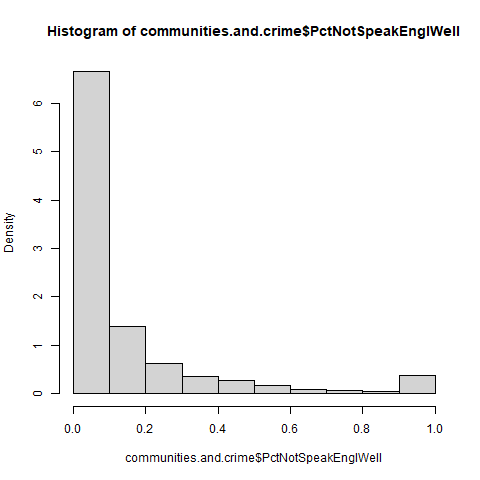
\includegraphics[width=0.45\textwidth]{beta/PctNotSpeakEnglWell_hist}
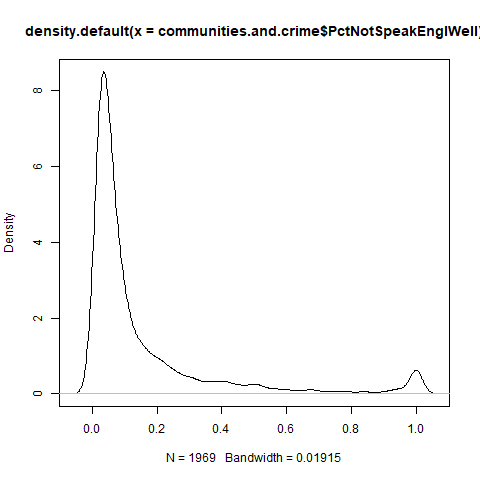
\includegraphics[width=0.45\textwidth]{beta/PctNotSpeakEnglWell_density}
\end{center}

\pagebreak
\section{Maximum Likelihood Estimation}
To find the MLE of the PctNotSpeakEnglWell, we first had to scale our data so it was within the beta family's support of $(0, 1)$: 
\begin{lstlisting}
  x[which(x == 0)] <- 0.0001  
  x[which(x == 1)] <- 0.9999
\end{lstlisting} 

We then defined our log-likelihood function as:
\begin{multline}
L(\alpha, \beta) = n \log{(\Gamma(\alpha+\beta))} - n \log{(\Gamma(\alpha))} - n \log{(\Gamma(\beta))} + \\
(\alpha - 1) \sum(\log(x)) + (\beta-1) \sum(\log{(1-x)})
\end{multline}

Using R's built-in mle() function, we utilized the \textit{negative} log-likelihood function to find the beta parameters of PctNotHsGrad.
\begin{lstlisting}
z <- mle(minuslogl = ll, start = c(list(alpha = 1), list(beta = 1)))
\end{lstlisting} 

\begin{center}
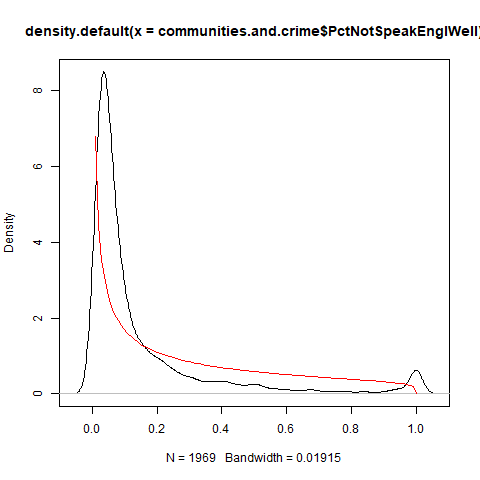
\includegraphics[width=0.45\textwidth]{beta/PctNotSpeakEnglWell_mle}
\end{center}

\pagebreak
\section{Method of Moments}
To find the MM-estimated density of PctNotSpeakEnglWell, we used the following function to predict the $\alpha$ and $\beta$ values:
\begin{lstlisting}
  mm <- function(x) {
    mu <- mean(x)
    var <- var(x)
    alpha <- mu * (mu * (1 - mu) / var - 1)
    beta <- (1 - mu) * (mu * (1 - mu) / var - 1)
    return(c(alpha, beta))
}
\end{lstlisting} 

\begin{center}
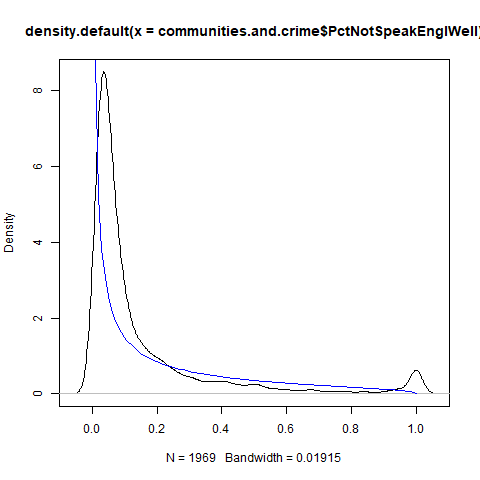
\includegraphics[width=0.45\textwidth]{beta/PctNotSpeakEnglWell_mm}
\end{center}

\section{Analysis}
The MLE and MM beta approximations of PctNotSpeakEnglWell exhibit notable differences from each other.
The MLE approximation decays slower than the actual data, while the MM approximation matches the tail of the data well, suggesting that it captures the decay behavior of the population density more accurately.



\chapter{Contributions}
\begin{itemize}
 \item \textbf{Steven Alvarado}: Report formatting, MLE of beta and MM of gamma and beta, finding potential distribution variables from datasets
 \item \textbf{Russell Chien}: Finding suitable variables from datasets, MLE and MM of exponential, transferring code and plots into latex report
 \item \textbf{Ruth Hailu}: Data analysis
\end{itemize}

\end{document}
